% Propósito: relacionar el desajuste de impedancias con la aparición de una
% onda reflejada en una interfaz ideal.
% Origen: R_p=(Z_02-Z_01)/(Z_02+Z_01) y R_I=|R_p|^2, ecuaciones
% \eqref{eq:u4-reflexion-presion} y el texto que la sigue.
% Esquema teórico para incidencia normal y medios sin pérdidas; no está a
% escala ni representa una medición.
% Descripción accesible: una onda llega desde el medio 1 a una interfaz
% vertical. Allí se divide en una onda reflejada que vuelve al medio 1 y una
% onda transmitida que avanza por el medio 2. Debajo se indica que la
% diferencia entre las impedancias determina el coeficiente de reflexión.
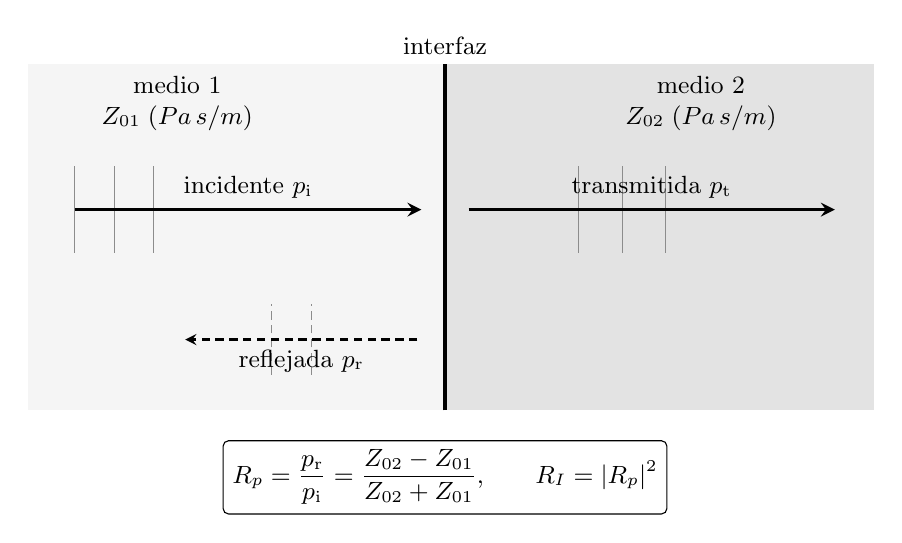
\begin{tikzpicture}[font=\small,>=stealth,x=1cm,y=1cm]
    \fill[black!4] (0.45,0.75) rectangle (5.75,5.15);
    \fill[black!11] (5.75,0.75) rectangle (11.20,5.15);
    \draw[very thick] (5.75,0.75) -- (5.75,5.15);
    \node[above] at (5.75,5.15) {interfaz};

    \node[align=center] at (2.35,4.65)
        {medio 1\\\(Z_{01}\;(\text{Pa}\,\text{s}/\text{m})\)};
    \node[align=center] at (9.00,4.65)
        {medio 2\\\(Z_{02}\;(\text{Pa}\,\text{s}/\text{m})\)};

    \foreach \x in {1.05,1.55,2.05}{
        \draw[black!45] (\x,2.75) -- (\x,3.85);
    }
    \foreach \x in {3.55,4.05}{
        \draw[black!45,densely dashed] (\x,1.20) -- (\x,2.10);
    }
    \foreach \x in {7.45,8.00,8.55}{
        \draw[black!45] (\x,2.75) -- (\x,3.85);
    }

    \draw[->,very thick] (1.05,3.30) -- (5.45,3.30)
        node[midway,above] {incidente \(p_\mathrm{i}\)};
    \draw[->,thick,densely dashed] (5.40,1.65) -- (2.45,1.65)
        node[midway,below] {reflejada \(p_\mathrm{r}\)};
    \draw[->,very thick] (6.05,3.30) -- (10.70,3.30)
        node[midway,above] {transmitida \(p_\mathrm{t}\)};

    \node[draw,rounded corners=2pt,fill=white,align=center] at (5.75,-0.10)
        {\(\displaystyle R_p=\frac{p_\mathrm{r}}{p_\mathrm{i}}
          =\frac{Z_{02}-Z_{01}}{Z_{02}+Z_{01}}\),\qquad
          \(\displaystyle R_I=|R_p|^2\)};
\end{tikzpicture}
